\subsubsection{Zeek}

According to \cite{strand_2022} Zeek (previously known as Bro) is an intrusion detection system that differs from others in that it focuses on network analysis. Unlike rules-based engines, which are meant to identify exceptions, Zeek searches for dangers and generates warnings. Zeek is an open-source, passive network traffic analyser. Zeek is widely used by operators as a network security monitor (NSM) \cite{electronics11050679} to aid in the investigation of suspicious or malicious behaviour. Zeek also provides support for a broad variety of traffic analysis activities outside of the security area, such as performance assessment and troubleshooting.
Extracting data from HTTP sessions, detecting malware by interacting with external registries, reporting vulnerable versions of software visible on the network, recognising popular online apps, detecting SSH brute-forcing, checking SSL certificate chains, and much more are all included into Zeek. \ref{prosncons}\\

\textit{Zeek - Malware detection using Zeek IDS}

As we know that Zeek is an open source Intrusion detection system which is primarily used detection of malwares and suspicious activities over the network. Zeek also work as a network monitoring tool for analysis of traffic. Even though Zeek does offer common capabilities like signature-based intrusion detection systems (IDS), its scripting language allows for a far wider range of very varied techniques to uncovering harmful activities. Anomaly identification, semantic misuse detection, and behavioral analysis are all examples of this. Intrusion detection using Zeek goes beyond typical signature-matching, yet the system still includes a comparable signature engine that can be used in the same way as previous systems. In addition, Zeek employs a flexible signature language of its own.\\
\\
\textit{Zeek - Architecture for detection of malware and malicious activities.}

As it examines network traffic, it looks for anomalies. Zeke is a fully functioning IDS, but not a full-fledged IPS. Only UNIX-like platforms are supported by Zeek Figure: \ref{fig:zeek_architecture} depicts the structure of Zeek. In addition to libpcap and the Event Engine, it also includes the Policy Script Interpreter.\\ 
\\
\begin{figure}[h]
    \centering
    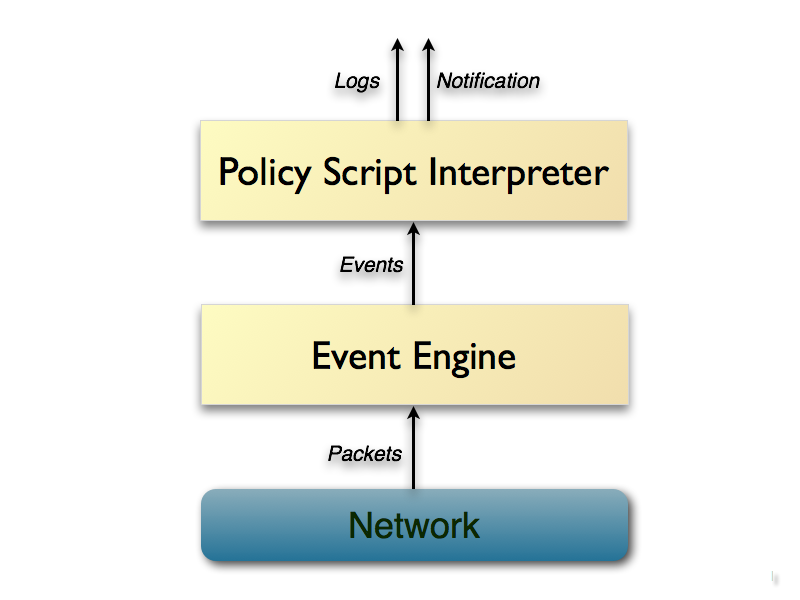
\includegraphics[width=0.5\textwidth]{images/zeek_architecture.png}
    \caption{Zeek Architecture \cite{Zeek2019}}
    \label{fig:zeek_architecture}
\end{figure}


\textit{Libpcap:} Zeek captures network packets using the libpacap packet capture library. Insignificant network traffic \cite{SHIMEALL2014253} is put under stress by this. 
\\
\textit{Event Engine:} Libpcap sends filtered traffic to the event engine. IP header checksum verification is one of the integrity checks performed by this layer to ensure that packets are properly generated. As a result, the network layer analyzer can access the complete IP packet. It communicates with the policy layer through events. 

\textit{Policy Script Interpreter:} Zeek policy scripts (rules) are written in a unique Zeek language that does not depend on standard signature detection. It examines the network to look for anomalies.\\
\\
\textit{Zeek - A Powerfull Malware Detector}
\\
Because of Zeek's ability to identify deception attacks as well as attacks concealed by normal TCP segmentation, Zeek-ids can do application-level deep packet inspection, Zeek can discover and analyze tunnels, and Time Machine, a high-performance packet bulk recorder with a Zeek interface, may boost forensic capabilities.  By using Zeek IDS we can easily detect different types of malware of different categories because of its anomaly based interpreter which reads the behavior of packet and analyze it.  Based on the architecture of Zeek IDS yes it is capable of detecting ransomware attacks \cite{Bhosale2015}. 

Zeek is a powerful tool for detection of malware and malicious activities because of its anomaly based detection features \cite{Haas2020ZeekOsqueryHC}. Features of Zeek makes it valuable and perfect for detecting anomalies and malware . Features of Zeek which makes it detect malwares at high efficiency are:\\

\begin{itemize}
    \item It gathers, analyses and correlates log data. 
    \item Searches for system alterations like those made by rootkits. 
    \item Automated response actions may be initiated by an active reaction. 
    \item Alerts that may be customised and sent in real time \\
\end{itemize}

As discussed, zeek is a very powerful tool for detection of malwares but zeek some of the drawbacks of zeek is that it does not provide any GUI support and is difficult to deploy so its deployment in small businesses without an dedicated IT team is difficult. 
 